\section{Pre processing}
\begin{figure}[ht]
    \centering
    \begin{subfigure}{0.4\linewidth}
        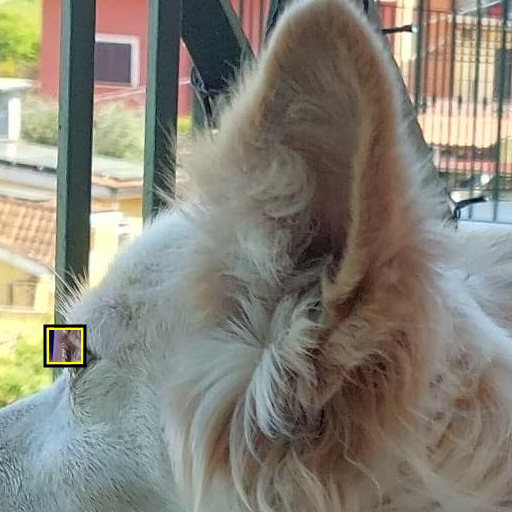
\includegraphics[width=\linewidth]{Figures/example_square.png}
    \end{subfigure}
    \hspace{2cm}
    \begin{subfigure}{0.4\linewidth}
        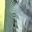
\includegraphics[width=\linewidth]{Figures/example_detail.png}
    \end{subfigure}
    \caption[Pixel grid detail]{Image detail.}
    \label{fig:example_detail}
\end{figure}

%La digitalizzazione delle immagini è un passo fondamentale per preparare le opere d'arte alle analisi che verranno effettuate. Per comprendere appieno il funzionamento di queste trasformazioni, è importante acquisire una conoscenza approfondita del processo attraverso cui un'opera pittorica viene catturata da una macchina fotografica e successivamente digitalizzata in un dispositivo elettronico.
Digitising images is a fundamental step in preparing the data set for analysis. To fully understand how these transformations work, it is important to understand the process by which a work of art is captured by a camera and then digitised in an electronic device.

\paragraph{Definition of image: from the real world to the virtual world}
%Gli artisti dell'antichità utilizzavano varie tecniche, come la camera oscura e i principi della geometria proiettiva, per rappresentare i paesaggi in modo realistico. Durante il Rinascimento, hanno ulteriormente perfezionato questi metodi con strumenti come la camera lucida, mostrando una comprensione matematica avanzata in opere d'arte come la Scuola di Atene di Raffaello.\begin{toDo} citare fonte \end{toDo}.
Artists of antiquity used various techniques, such as the camera obscura and the principles of projective geometry, to represent landscapes realistically. During the Renaissance, they further refined these methods with tools such as the camera lucida, showing advanced mathematical understanding in works of art such as Raphael's School of Athens.\footnote{for more about camera obscura, see\newline\url{https://www.academia.edu/28360703}}

%\noindent L'invenzione della fotografia nel $1826$, in concomitanza con il movimento artistico del Realismo, segnò un momento fondamentale nella storia dell'arte visiva. La fotografia, con la sua capacità di rappresentare la realtà in modo oggettivo, divenne uno strumento sempre più utilizzato dagli artisti. L'avanzamento delle conoscenze in ottica e chimica portò alla creazione della fotografia analogica \begin{toDo} citare fonte e inserire immagine \end{toDo}.
\noindent The invention of photography in $1826$, in conjunction with the art movement of Realism, marked a fundamental moment in the history of visual art. Photography, with its ability to represent reality objectively, became a tool increasingly used by artists. The advancement of knowledge in optics and chemistry led to the creation of analogue photography.\footnote{for more about history of photography, see\newline\url{https://marcocrupi.it/2011/03/come-la-fotografia-cambio-larte-storia.html}}
\begin{figure}[ht]
    \centering
    \begin{subfigure}[t]{0.4\linewidth}
        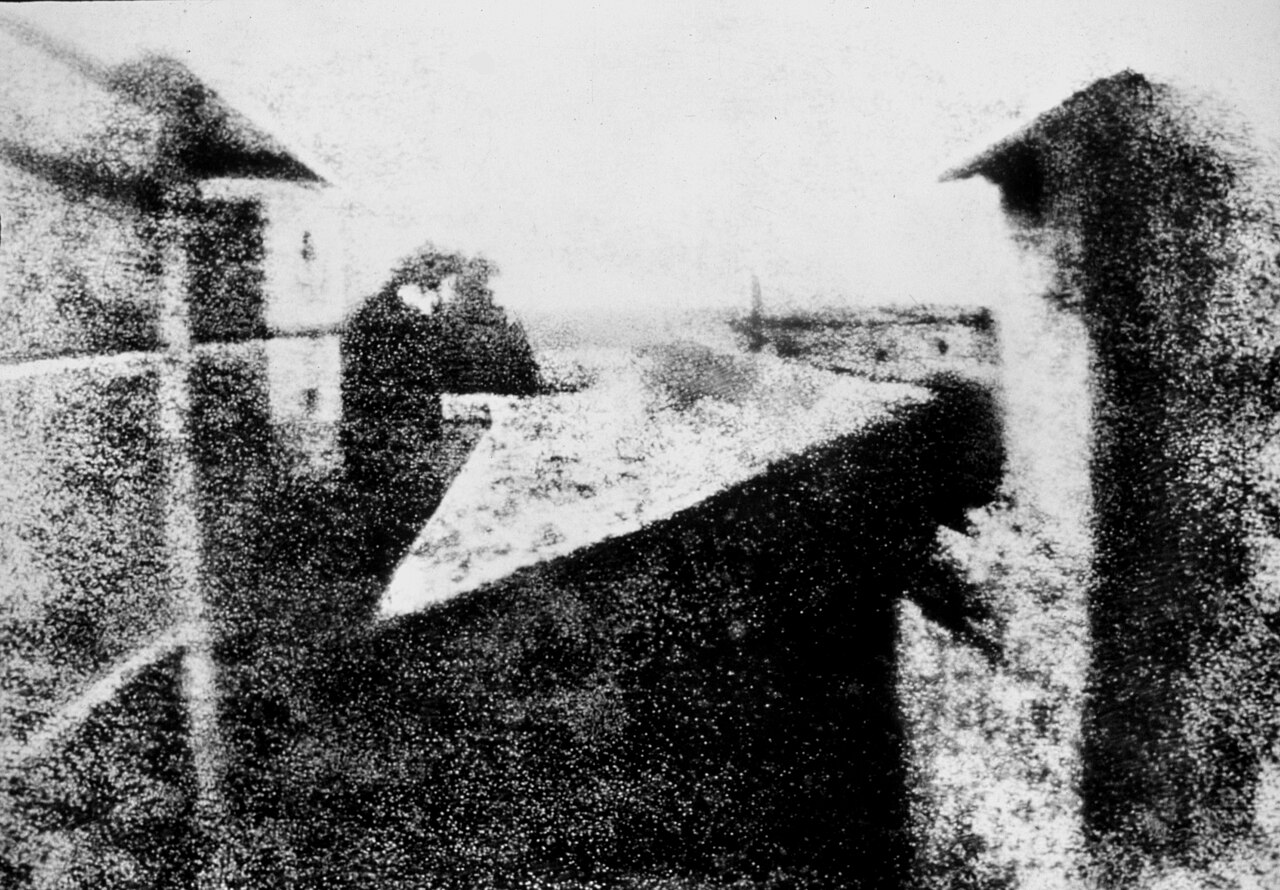
\includegraphics[width=\linewidth]{Figures/FotoStoria.jpg}
        \caption{'View from the Window at Le Gras', Joseph Nicéphore Niépce, c.1826, Heliography, Harry Ransom Center, University of Texas at Austin, USA\cite{FirstPhoto}.}
    \end{subfigure}
    \hspace{2cm}
    \begin{subfigure}[t]{0.4\linewidth}
        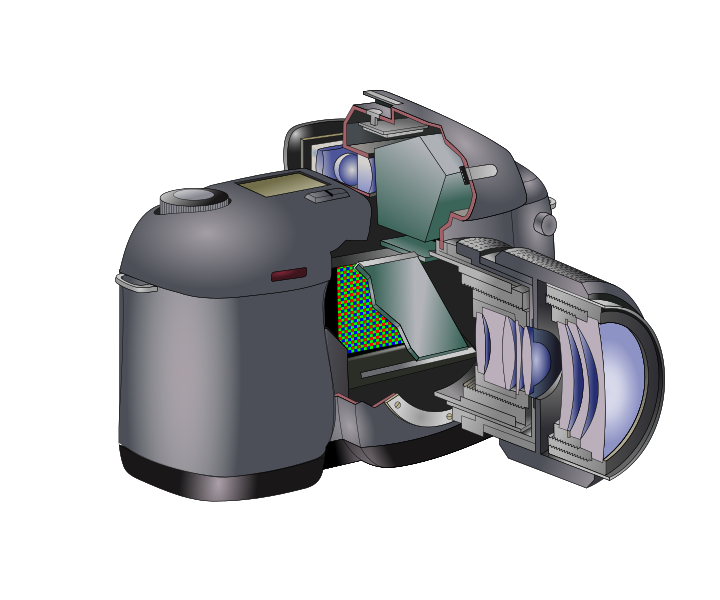
\includegraphics[width=\linewidth]{Figures/digitalcamera.png}
        \caption{Illustration of digital camera\cite{Reflex}.}
    \end{subfigure}
\end{figure}

%\noindent Nel corso degli anni ottanta, con l'avvento della tecnologia informatica, la fotografia digitale divenne una realtà. Il funzionamento di base rimase simile alle tecniche precedenti, ma con l'aggiunta di un nuovo processo di digitalizzazione. Invece di essere impressa su una superficie fotosensibile, l'immagine viene catturata da una griglia di sensori ottici e digitalizzata come una matrice di colori, con ogni componente chiamata "pixel" \begin{toDo} inserire fonte e immagine \end{toDo}.
\noindent During the 1980s, with the advent of computer technology, digital photography became a reality. The basic operation remained similar to previous techniques: instead of being printed on a photosensitive surface, the image was captured by a grid of optical sensors and digitised as a matrix of colours, with each component called a pixel.

%\noindent Il concetto di riproduzione dei colori non è nuovo, e già nel $1855$ James Clerk Maxwell lavorò su questo tema, introducendo il modello di colore \gls{rgb}, ancora oggi ampiamente utilizzato. Questo modello codifica ogni colore con tre numeri reali in un intervallo tra $0$ e $1$. Tuttavia, per scopi informatici, si è convenuto di rappresentare i $3$ valori di un colore con numeri interi compresi tra $0$ e $255$ \begin{toDo} inserire fonte per lavoro di Maxwell \end{toDo}. In questo modo, un'immagine digitale diventa una matrice di triple, rappresentando i valori dei pixel nei tre canali di colore \gls{rgb}.
\noindent The concept of colour reproduction is not new and as early as $1855$ James Clerk Maxwell worked on this subject, introducing the colour model \gls{rgb}, which is still widely used today (see \cite{MaxWell_Colours}). This model encodes each colour with three real numbers in an interval between $0$ and $1$. However, for computing purposes, it was agreed to represent the $3$ values of a colour with integers between $0$ and $255$. In this way, a digital image becomes a matrix of triples, and each pixel is represented with the three colour channels \gls{rgb}.

\subsection{Grayscale reduction}
The quantisation of colours is expressed in $3$ channels \gls{rgb}, each with an integer value between $0$ and $255$. The choice of these $3$ colours is not arbitrary; it derives from a physiological feature of human vision. Our perception of colour is determined by photoreceptor cells in the eye called cones, of which there are three types: S-cones, M-cones and L-cones. These cones are sensitive to wavelengths that approximately correspond to blue, green and red light respectively.

\noindent This model of colour representation is therefore deeply rooted in the way our visual system works, rather than in the physical reality of light. For example, when we see yellow, it is the result of the simultaneous activation of both M and L cones, which our brain interprets as a pure yellow colour. This perception is not a direct consequence of the physical properties of light, but rather a result of our brain's processing. Similarly, the colour magenta does not have a single wavelength in the visible spectrum, but is perceived when our brain combines stimuli from both red and blue wavelengths. These examples illustrate that colour perception is a subjective phenomenon in which the brain combines signals in a way that does not always reflect a direct physical counterpart.

\noindent This subjective nature of colour perception means that our representation of colour space is influenced more by neurological processes than by physical reality. While physically we might think of colour as occupying a continuous, structured space (e.g. a cone or cylinder in RGB representation), the actual experience of colour varies between individuals. For example, people with colour blindness may perceive certain colours differently due to differences in their cones. In addition, cultural differences can also affect perception: the Himba people of Namibia, for example, can distinguish between shades of green that many others cannot, while they may have difficulty distinguishing green from blue\footnote{For more about Himba people, see \url{https://psycnet.apa.org/record/2000-05104-005}}.

\noindent Given this subjective interpretation, the classification of colours often goes beyond a purely scientific approach. In contexts such as art, where perception and expression are key, it is often more useful to refer to colour spaces such as \gls{hsl}, which represent hue, saturation and lightness, rather than the more physically oriented \gls{rgb}. These spaces provide a more intuitive way of describing how colours relate to each other in terms of what we actually perceive.

\noindent Greyscale reduction builds on this understanding of colour perception. It involves reducing the image to the brightness component only, effectively removing hue and saturation. There are several techniques to achieve this. One common method is to take a weighted average of the three RGB channels, with the weights chosen to reflect the varying sensitivity of the human eye to different colours. Another approach is to average between the maximum and minimum intensity channels. Whatever the method, the aim is to create a representation of the image that retains luminance information while discarding colour, thus simplifying the visual data while retaining the essence of light intensity.

\begin{figure}[h]
    \centering
    \begin{subfigure}[t]{0.4\linewidth}
        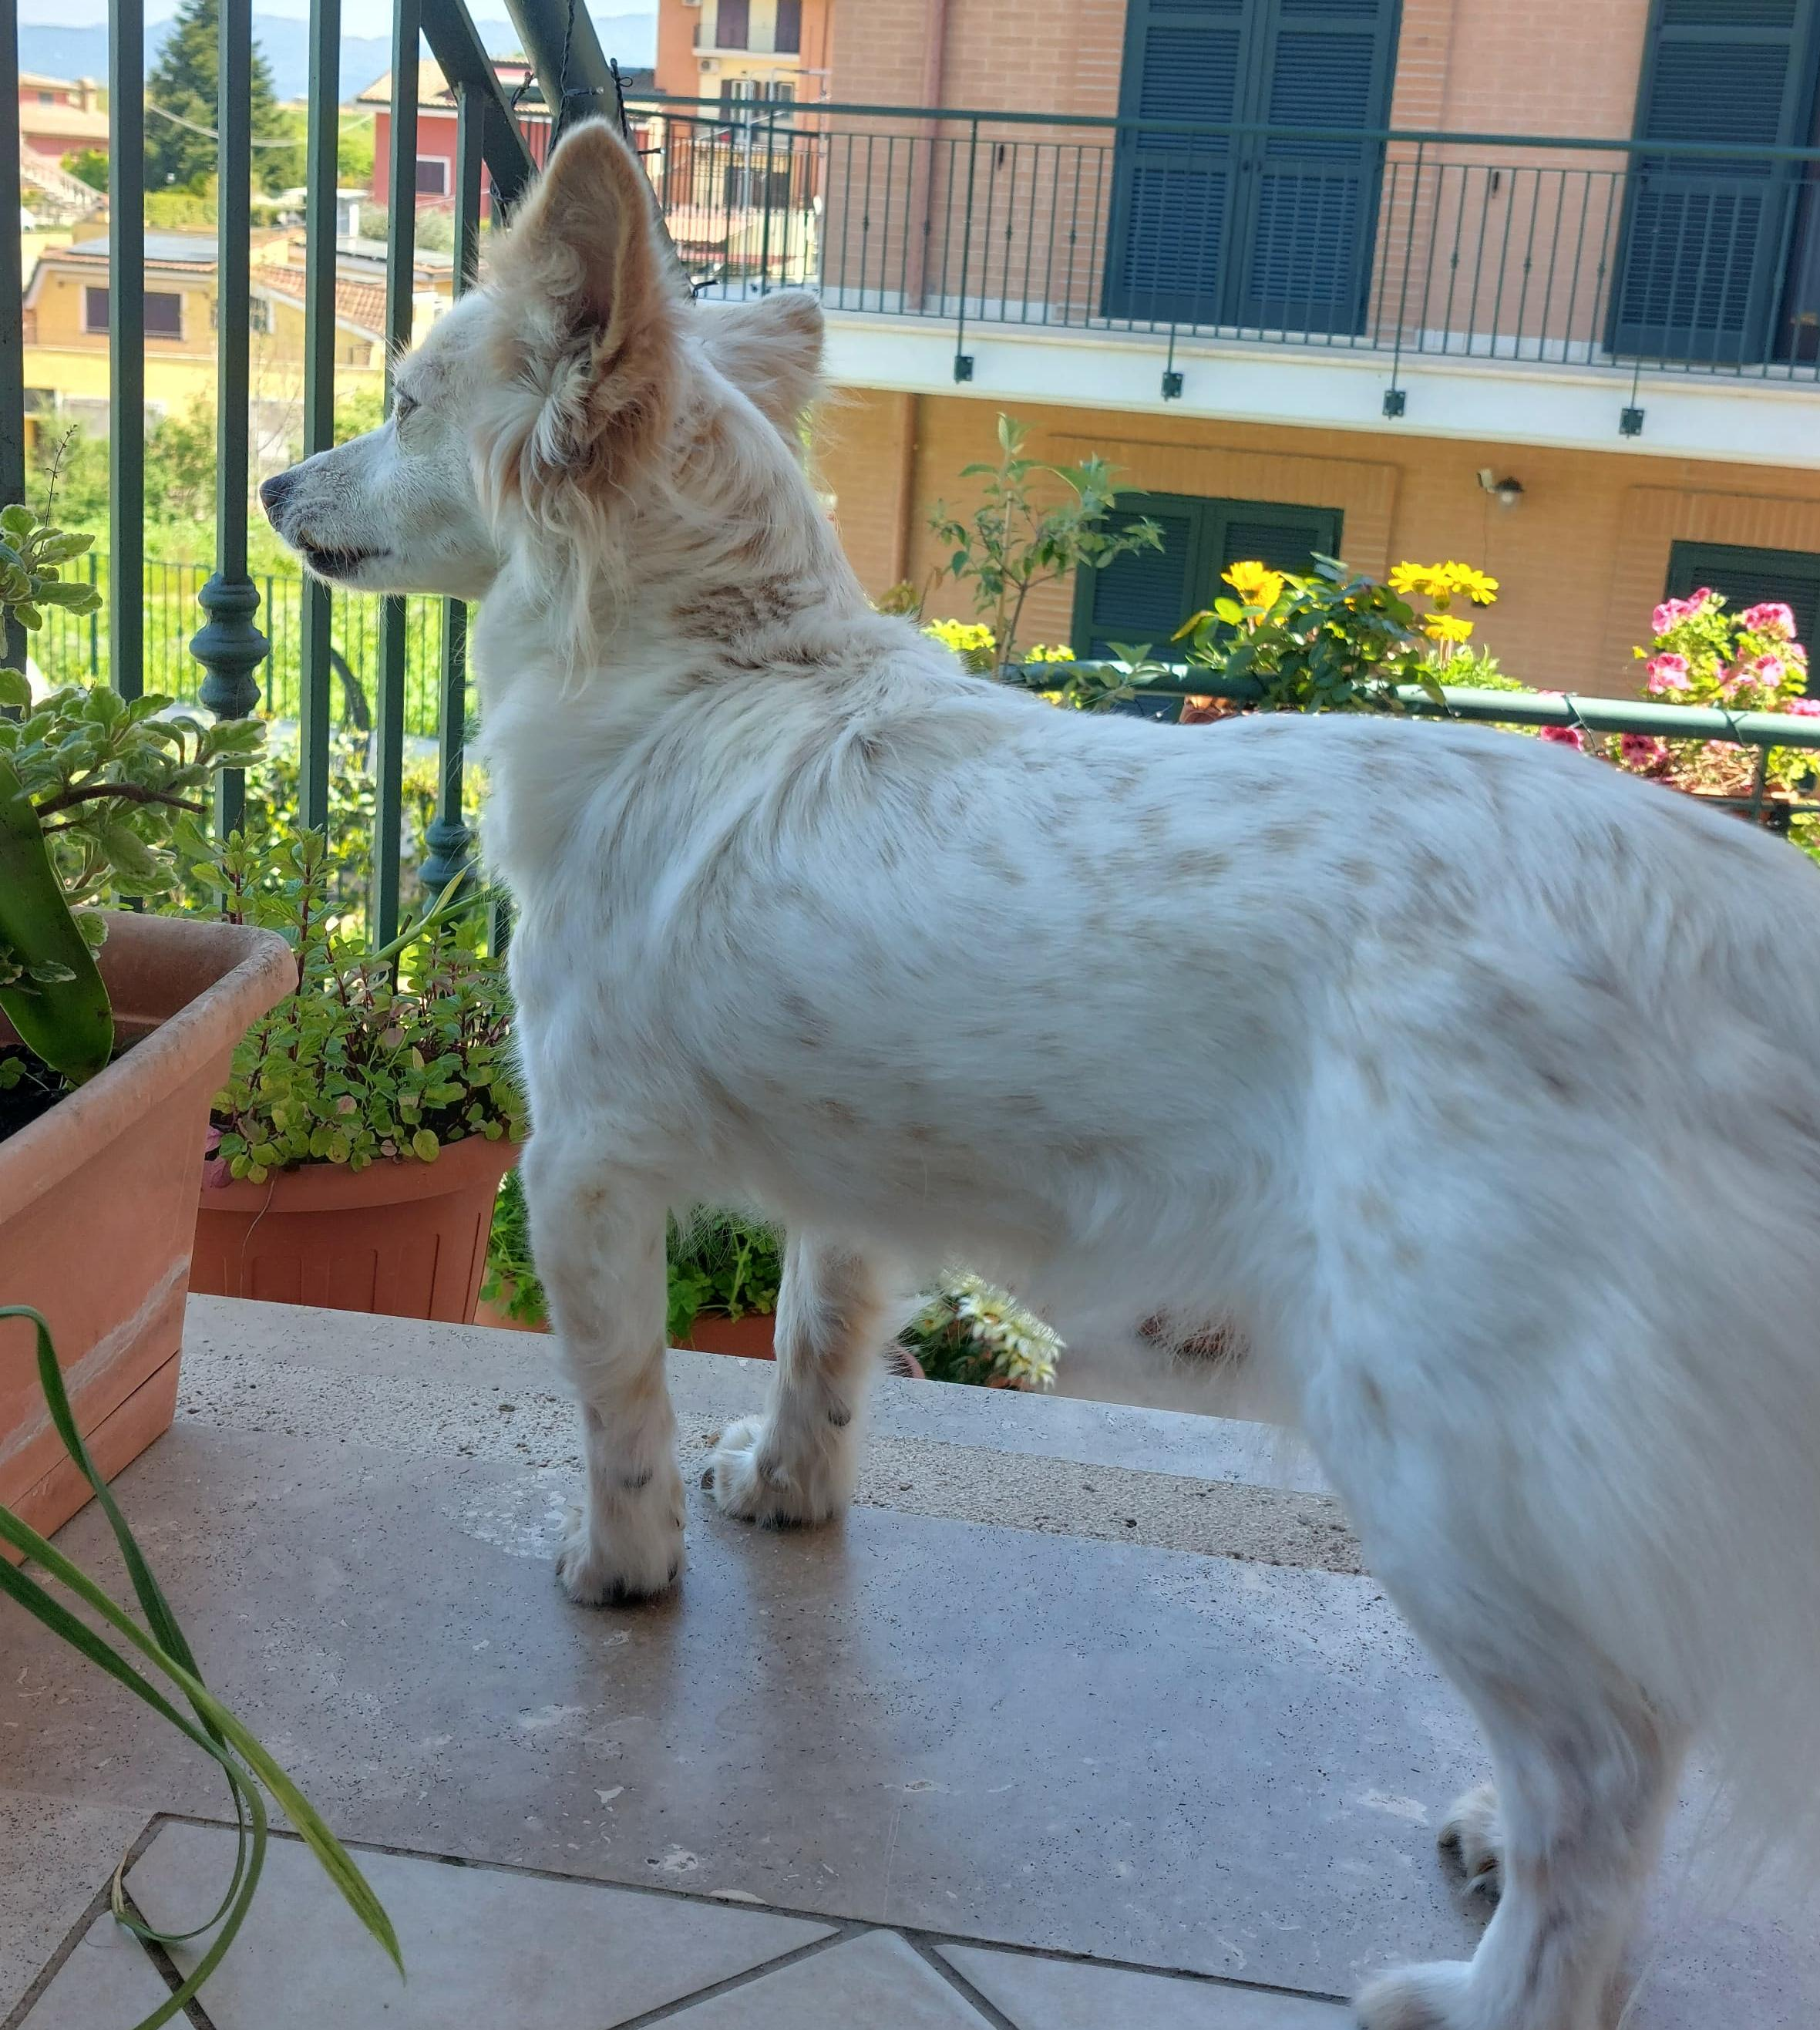
\includegraphics[width=\linewidth]{Figures/example.jpeg}
    \end{subfigure}
    \hspace{2cm}
    \begin{subfigure}[t]{0.4\linewidth}
        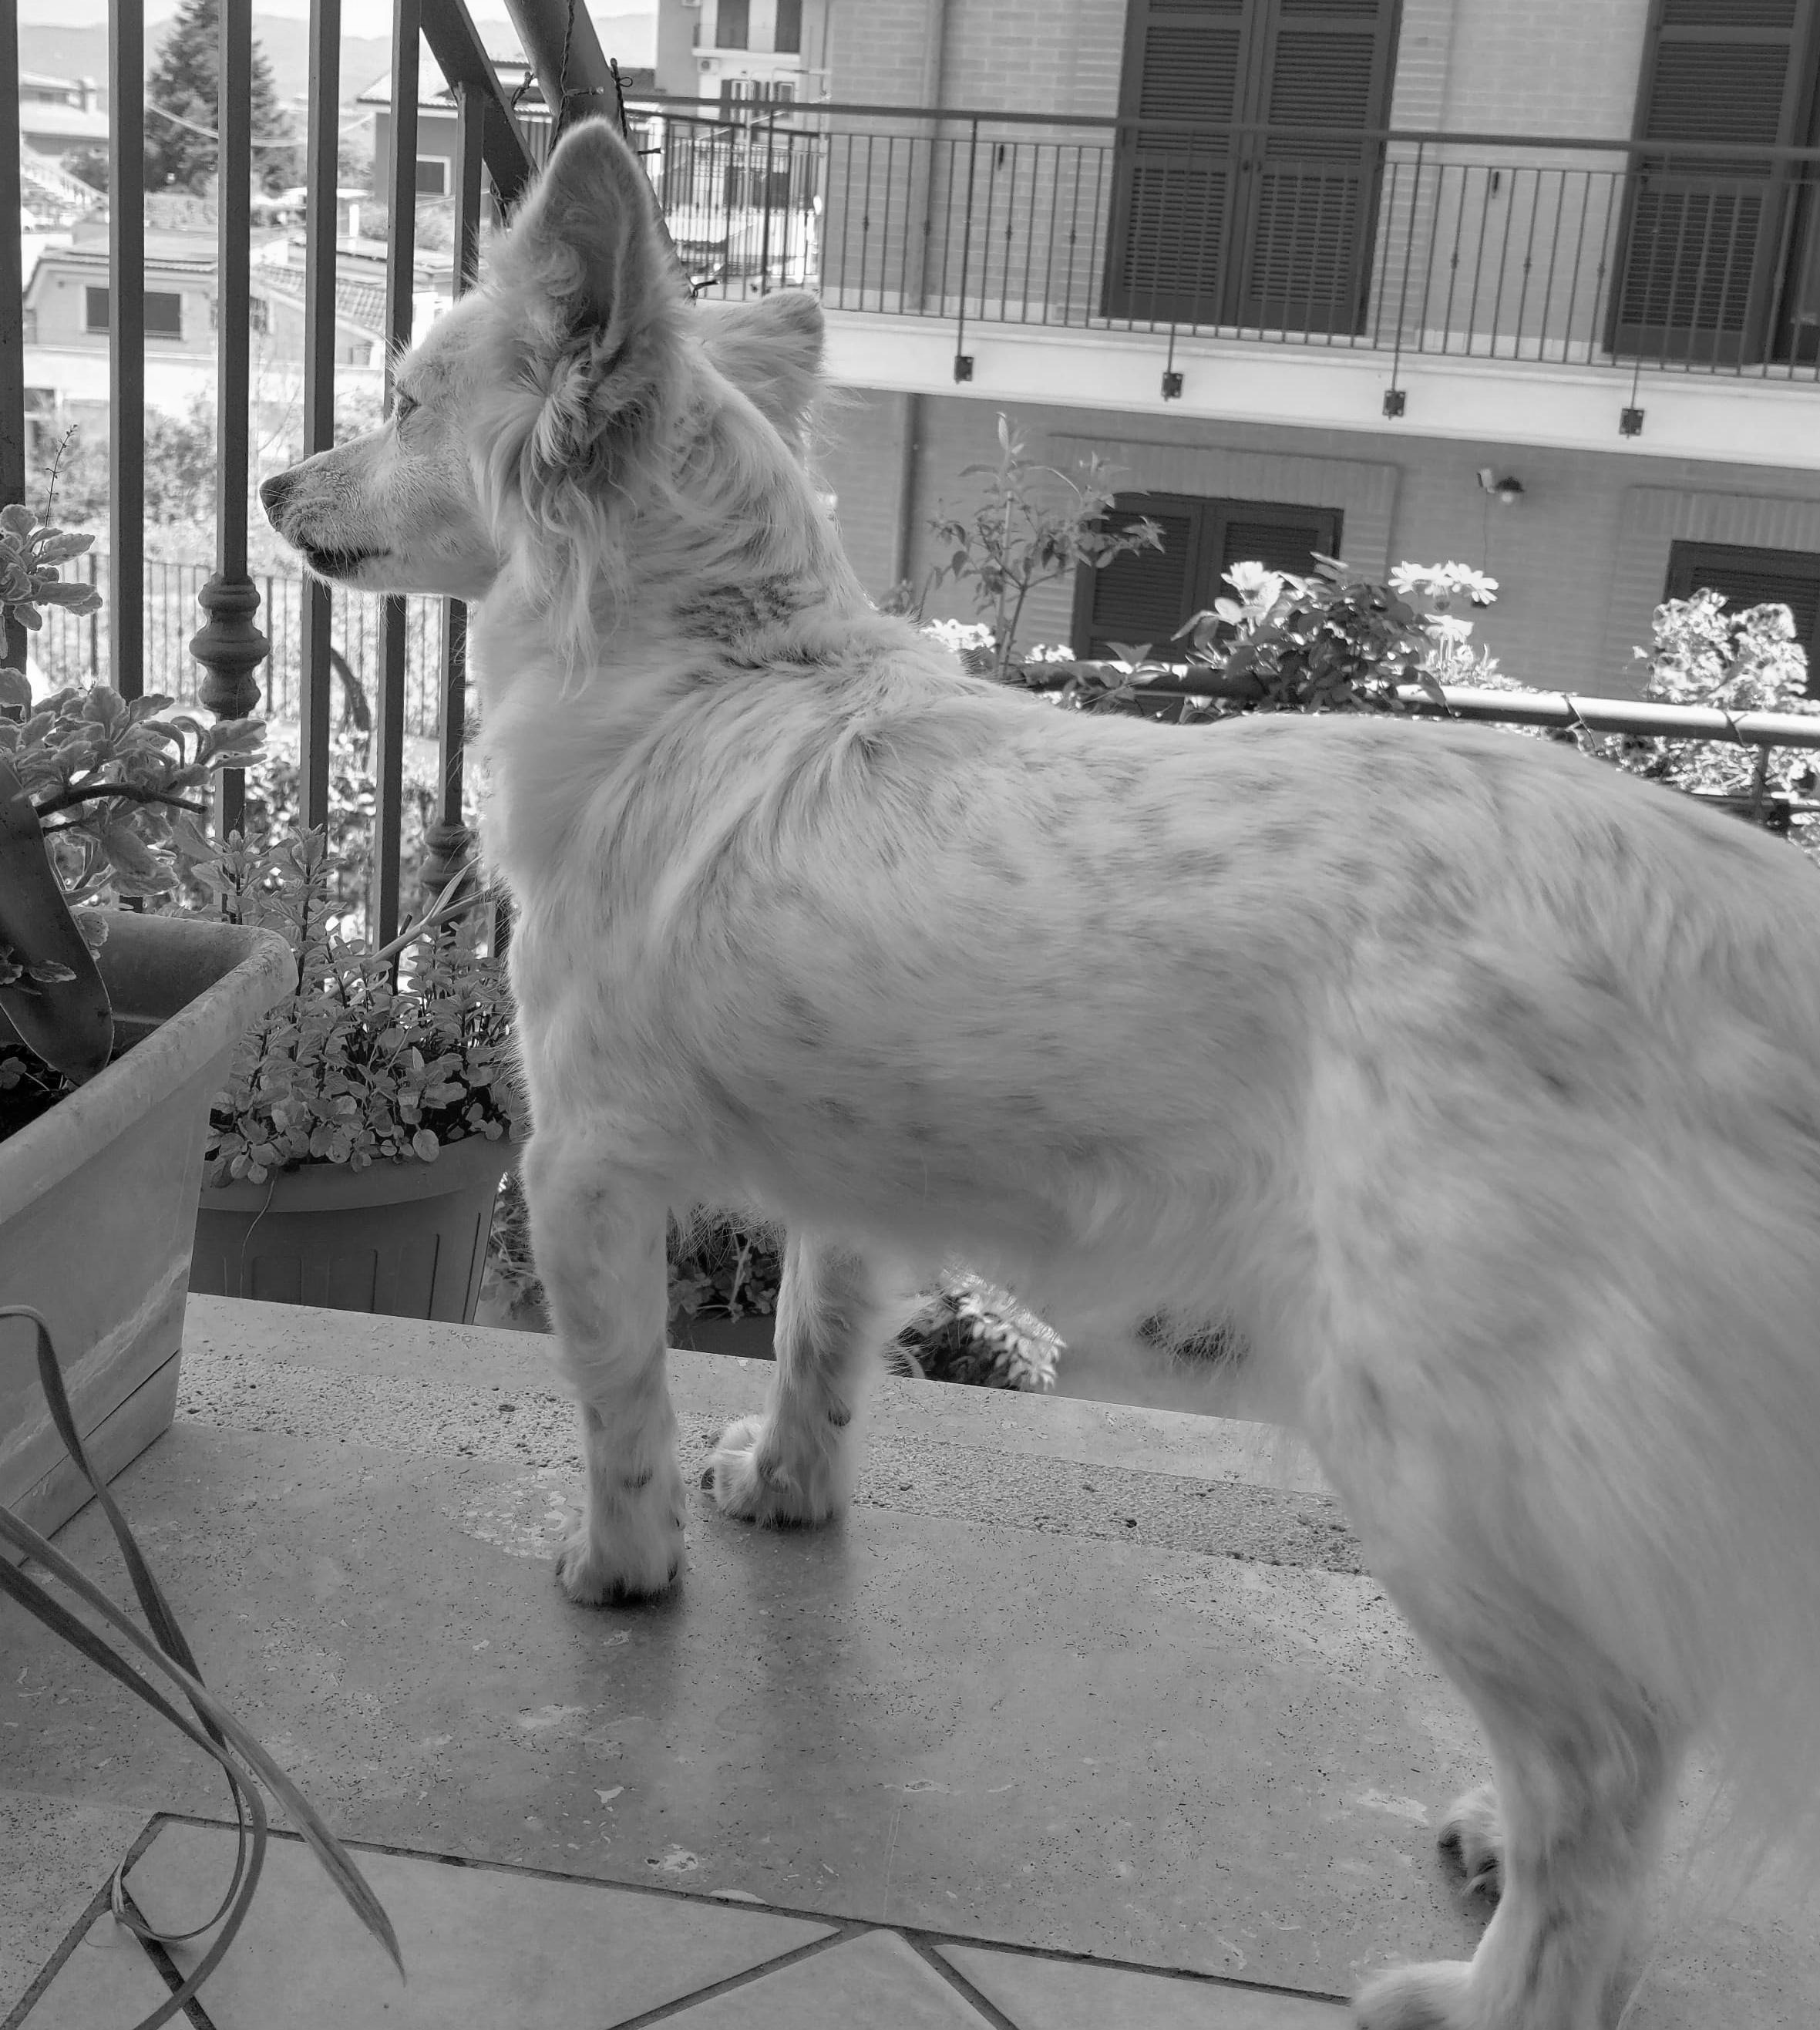
\includegraphics[width=\linewidth]{Figures/example_gray.jpeg}
    \end{subfigure}
\end{figure}
\subsection{Removing squares}
    One of the main challenges in processing and collecting the dataset concerns the cleanliness of the images, which can have significant impurities, such as the presence of squares on the sheets. It is essential to remove or mitigate these elements so that they blend in with the background and do not interfere with the analysis. Initially, the use of static techniques such as thresholding or the application of specific kernels to recognise the squares was considered. However, such techniques risked compromising the author's writing by erasing details. For this reason, it was decided to use compression techniques to detect patterns, since squares constitute a highly visible pattern that is more easily distinguishable by the machine than human handwriting.

    \paragraph{\gls{svd}}
    A first test involved examining the predominant patterns by means of a decomposition \gls{svd}. The image can be viewed as a matrix $H \times W$ of real values and can be decomposed into the product:
    \[
    	U\Sigma V^H = M
    \]
    where $M$ represents the image, $U$ and $V$ are unitary matrices ($UU^H = I$, same for $V$), $V^H$ is the Hermitian of $V$, and $\Sigma$ is a matrix $H \times W$ with only non-negative values along the diagonal, called singular values.\
    It is possible to obtain a less detailed version of $M$ by cancelling some singular values of $\Sigma$, thus ignoring the contribution of certain patterns. It was observed that the predominant pattern (associated with the largest singular value) concerns squares, but its removal does not completely solve the problem, requiring the elimination of further patterns. The result obtained is encouraging, but entails a loss of information from human handwriting, as it too is present among the major patterns identified.

    \begin{toReview}
    \noindent This issue arises from the nature of the \gls{svd} decomposition. Since the method considers the image as a linear transformation, removing the dominant component is equivalent to removing the strongest eigenvector of the transformation. However, $M$ is not inherently a linear transformation, and even small isometric transformations of the image (e.g. rotations) can affect the result.

    \noindent An example is shown in \cref{fig:svd_counterexample} to illustrate this issue. The first row shows an ideal scan with perfectly vertical and horizontal lines. The second row shows the effect of a $1\degree$ rotation, where the grid remains visible despite the application of \gls{svd} compression. Finally, the third row shows stronger compression, highlighting that the grid remains while the handwriting fades.

    \begin{figure}[H] \centering \begin{subfigure}[t]{0.4\linewidth} 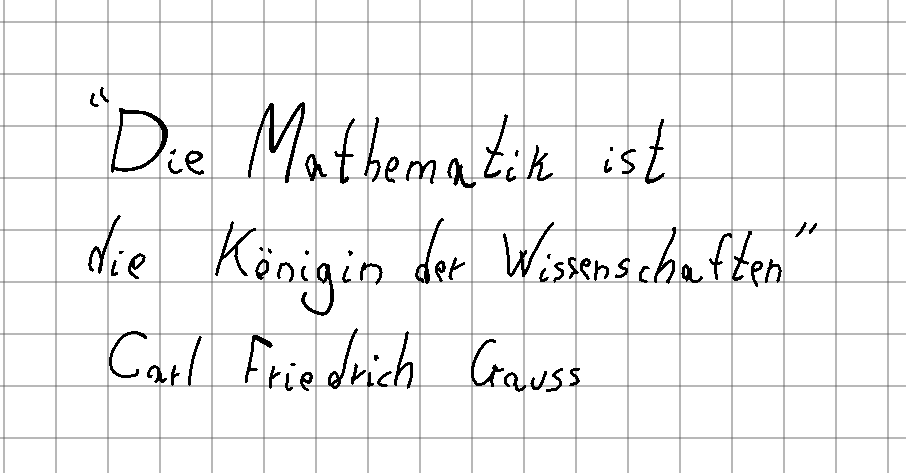
\includegraphics[width=\linewidth]{Figures/fraseGauss.png} \end{subfigure} \hspace{2cm} \begin{subfigure}[t]{0.4\linewidth} 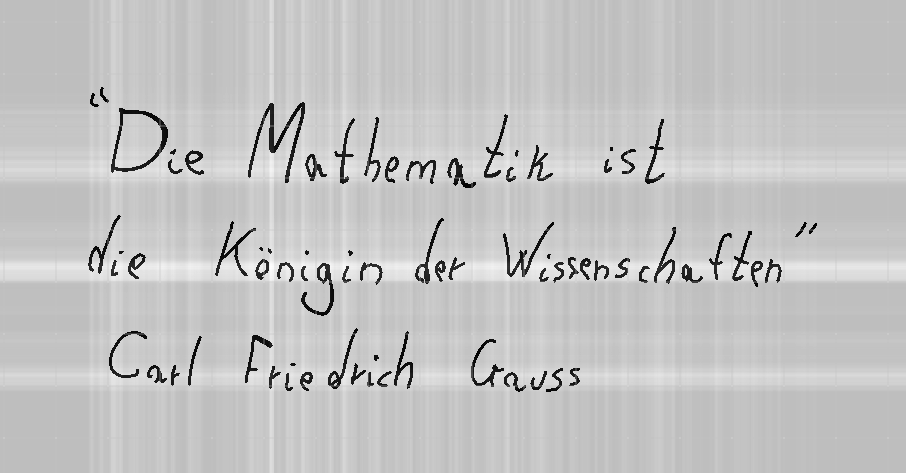
\includegraphics[width=\linewidth]{Figures/fraseGauss_compression.png} \end{subfigure} \par\vspace{1cm} \begin{subfigure}[t]{0.4\linewidth} 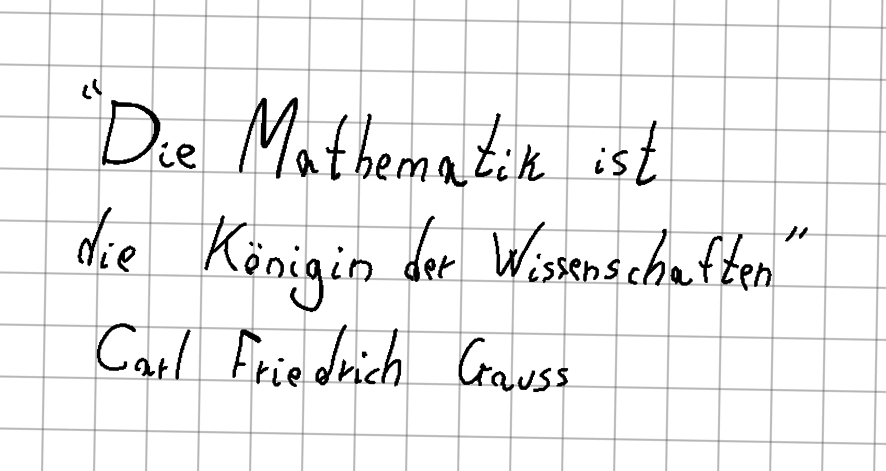
\includegraphics[width=\linewidth]{Figures/fraseGauss_rotated.png} \end{subfigure} \hspace{2cm} \begin{subfigure}[t]{0.4\linewidth} 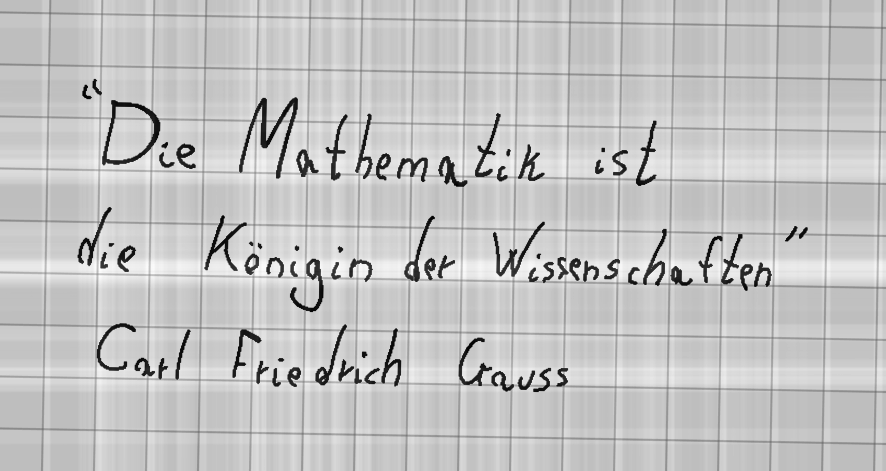
\includegraphics[width=\linewidth]{Figures/fraseGauss_rotated_compression.png} \end{subfigure} \par\vspace{1cm} \begin{subfigure}[t]{0.4\linewidth} 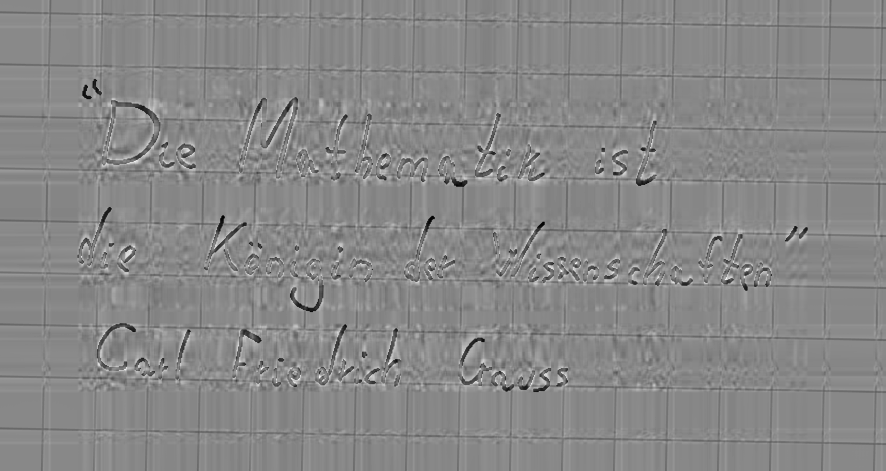
\includegraphics[width=\linewidth]{Figures/fraseGauss_compression20.png} \end{subfigure} \hspace{2cm} \begin{subfigure}[t]{0.4\linewidth} 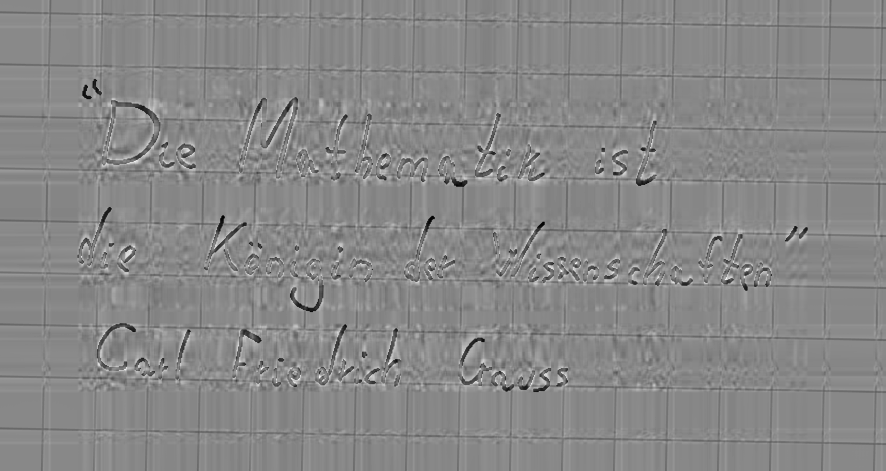
\includegraphics[width=\linewidth]{Figures/fraseGauss_compression20.png} \end{subfigure} \label{fig:svd_counterexample}\caption[Issues of \gls{svd} compression]{The first row shows an ideal scan with perfectly vertical and horizontal lines. The second row illustrates an imperfect scan with a $1\degree$ rotation, where the grid remains visible. The third row shows stronger compression, where the grid persists, but the handwriting fades.} \end{figure}
\end{toReview}

\paragraph{\gls{fft}}
    An alternative idea is to perform a harmonic analysis of the images using \gls{fft}. The squares are repeated with a specific frequency along the two dimensions of the sheet and thus one can exploit their regular nature compared to human handwriting, which is less repetitive. Thus, one exploits both the difference between the regular patterns of the squares and the irregular strokes of the handwriting, as well as a greater capacity for compression than a simple pixel-by-pixel analysis.

\begin{modified}
    \noindent To verify this idea, we run a \gls{fft} on test images: a virtual sheet with only squares and the same sheet with handwriting added to it. In the case of the unmarked sheet, frequencies with larger amplitudes are mainly found aligned along the $x$ and $y$ axes (\cref{fig:synthetic_grid_fft}). By adding handwriting, the primary frequencies characterizing the grid remain visible, even though additional frequencies introduced by the handwriting may partially overlap them (\cref{fig:synthetic_sign_fft}). To remove the squares, we filter out the frequencies of squares and reconstruct the image (\cref{fig:synthetic_clean_fft}).
\end{modified}

\begin{figure}
	\centering
	\begin{subfigure}[t]{\linewidth}
		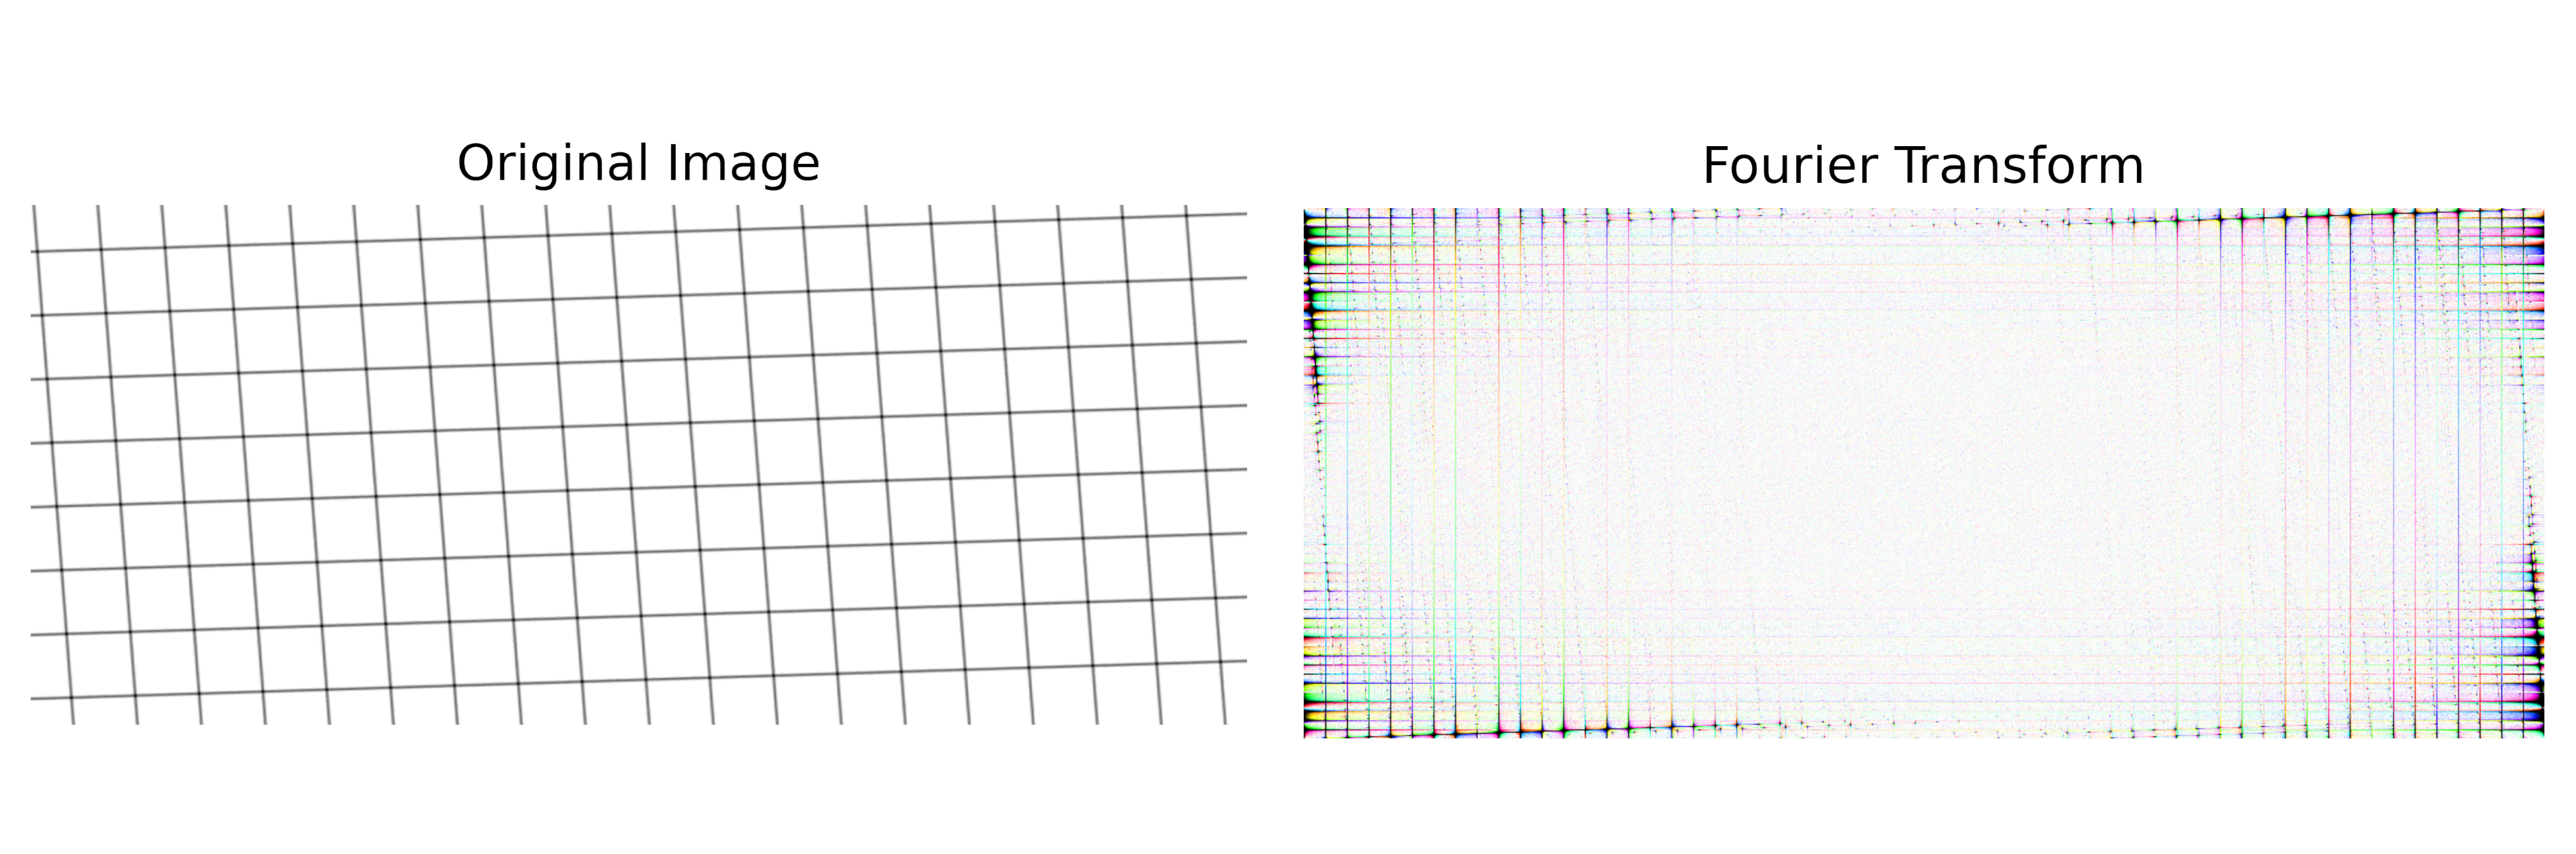
\includegraphics[width=\linewidth]{Figures/grid_fft.png}
		\caption{An imperfect scan can show a slightly rotated grid, as seen in the left image. On the right, the Fourier coefficients of the scanned image are displayed. The most significant frequencies, with high amplitudes, are highlighted in black.}
		\label{fig:synthetic_grid_fft}
	\end{subfigure}
	\begin{subfigure}[t]{\linewidth}
		\includegraphics[width=\linewidth]{Figures/test_fft.png}
		\caption{In this case, handwriting was superimposed. The frequencies of the grid remain visible despite the added handwriting.}
		\label{fig:synthetic_sign_fft}
	\end{subfigure}
	\begin{subfigure}[t]{\linewidth}
		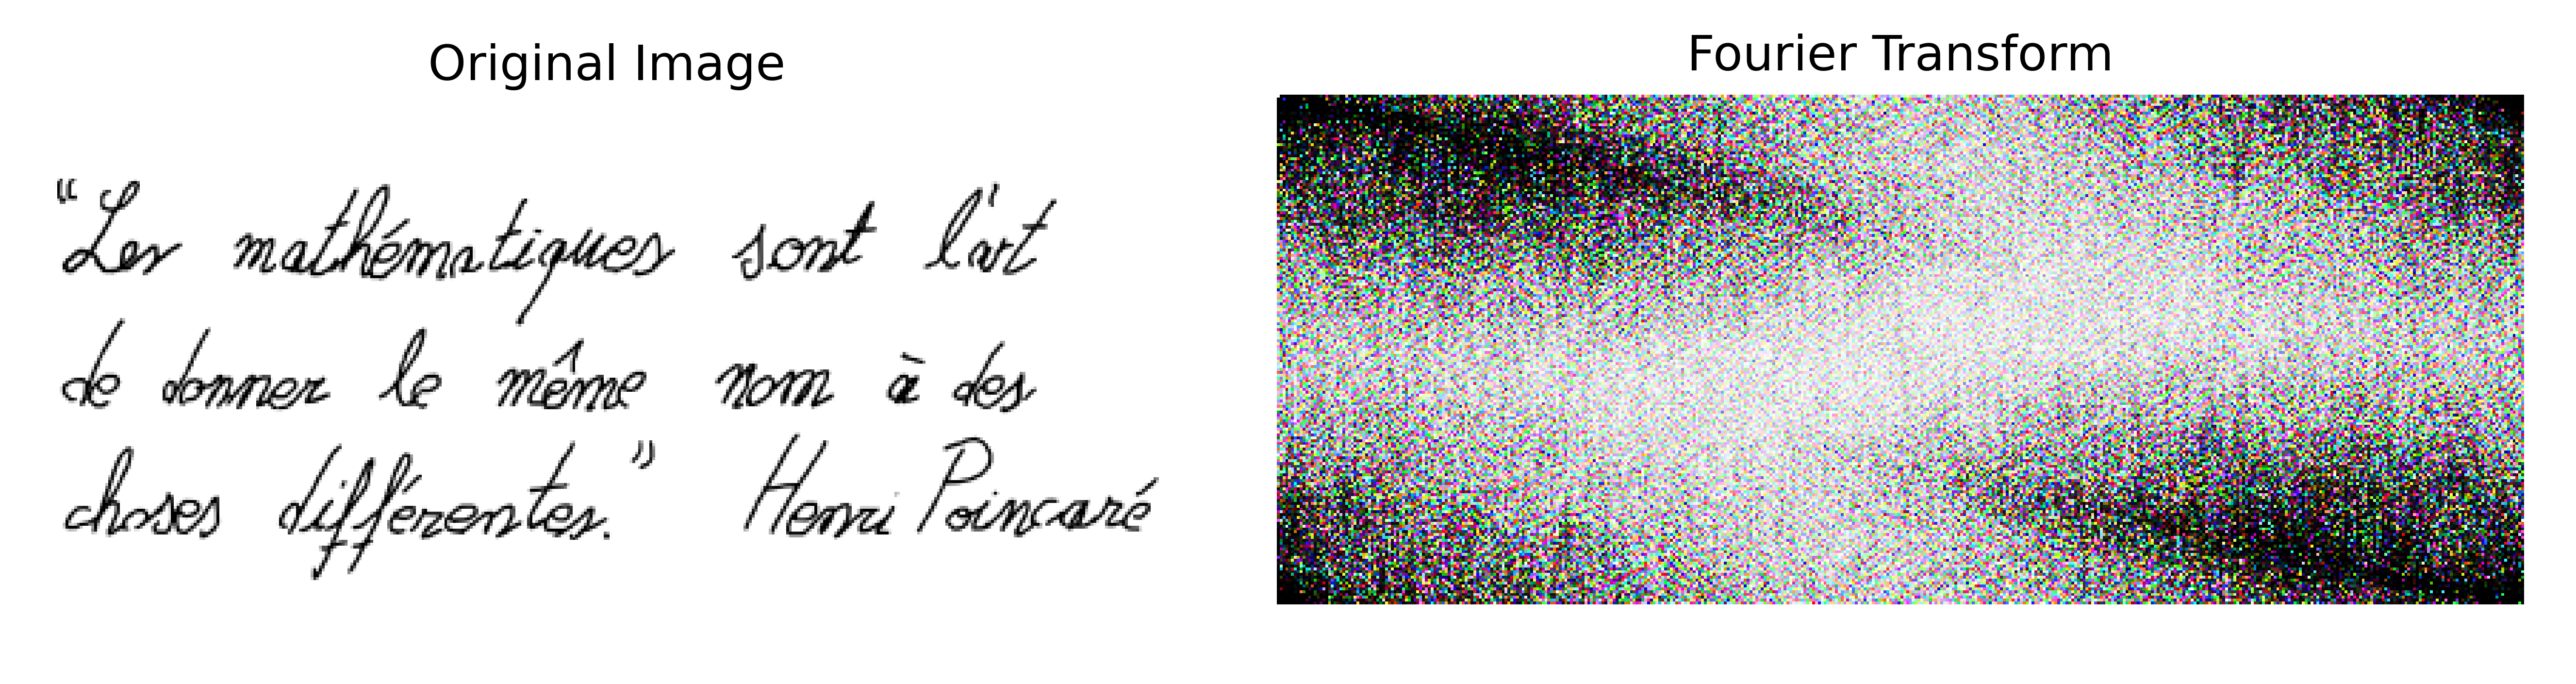
\includegraphics[width=\linewidth]{Figures/clean_fft.png}
		\caption{The cleaned handwriting, free from the grid, no longer shows the Fourier coefficients corresponding to the squares, as recurring patterns are absent.}
		\label{fig:synthetic_clean_fft}
	\end{subfigure}
	\caption[Synthetic FFT test]{Fourier coefficients of grayscale images are organized into matrices of complex numbers. Each component at coordinates $n,m$ has an amplitude and a phase that correspond to the respective frequencies $2\pi\frac{n}{N}$ and $2\pi\frac{m}{M}$, where $N$ and $M$ are the dimensions of the image. The phase is represented by hue, while amplitude is represented by brightness: darker pixels indicate higher amplitude.}
\end{figure}

    \noindent Empirically, by analysing $10$ randomly selected real images from the dataset, it was observed that the squares were successfully removed without damaging the lettering, cancelling out the amplitudes corresponding to the first $5\%$ percentile of the most significant frequencies.

	\begin{modified}
    \noindent After reconstructing the image using the \gls{fft}, a significant number of pixels took on intermediate shades of grey that weren't present before. This effect is likely due to the removal of specific frequency components during the filtering process. The reconstruction introduces a real-valued matrix, where some components have extreme positive or negative values. When the image is normalized to the $[0,1]$ range, the majority of pixel intensities are compressed into a narrower range of grey values, blending the background and the lettering. This normalization amplifies the loss of contrast, making it harder to distinguish important features from the unwanted noise.
	\end{modified}

	\noindent To reduce the effects of this distortion, we adopted a different colour normalisation approach to keep the grey values as close as possible to the original image. The main idea was to identify extremely light and extremely dark grey values in the original image and to expand the range of grey values in the reconstructed image to match them.

	\begin{modified}
    \noindent It was observed that, in the original image, pixels with a grey level below $0.2$ correspond to the lettering, while those with a grey level above $0.8$ represent the white background of the page. Using these thresholds, we count the number of dark pixels \(c_d\) and light pixels \(c_l\) in the original image. In the cleaned image, we then identify the $c_d$ darkest pixels and the $c_l$ lightest pixels to determine the new grey levels: $h_d$, below which all pixels are considered dark, and $h_l$, above which all pixels are considered light.

    \noindent To enhance the result of the \gls{fft} filtering, we adjust the grey levels of the cleaned image using a linear transformation. This transformation ensures that all pixels with a grey value below $h_d$ became black ($0$), and those above $h_l$ become white ($1$):
    \[
    	\texttt{new gray value} = \frac{\texttt{gray value} - h_d}{h_l - h_d}
    \]
    Finally, a clamp operation is applied to ensure all values remain within the range $[0,1]$:
    \[
    	\texttt{final gray value} = \begin{cases}
    		0 & \text{if } \texttt{new gray value} < 0, \\
    		1 & \text{if } \texttt{new gray value} > 1, \\
    		\texttt{new gray value} & \text{otherwise}
    	\end{cases}
    \]

    \noindent This operation, called \texttt{clamp}, ensures that the contrast between the lettering and the background is maximized, improving the overall quality of the cleaned image.

    \begin{algorithm}[h]
    	\caption[Cleaning procedure using \gls{fft}]{Cleaning procedure using \gls{fft}.\\
    		\begin{minipage}[t]{\linewidth}
    			\textsc{INPUT}
    			\begin{itemize}[noitemsep, topsep=0pt]
    				\item[$\mathcal{I}$:] Image as matrix $W\times H$ in gray scale
    				\item[$p$:] Fraction (or percentile) of the highest magnitudes to be considered significant
    				\item[$a$:] thresholds $(\min, \max)$
    			\end{itemize}
    			\textsc{OUTPUT} $\mathcal{I}_{\text{new}}$: Image as matrix $W\times H$ in gray scale
    		\end{minipage}
    	}
    	\begin{algorithmic}[1]
    		\Procedure{CleanFFT}{$\mathcal{I}, p, a$}
    		\State $\hat{\mathcal{I}} \gets \text{normalize}\left(\mathcal{I}\right)$ \Comment Normalize the gray level of image's pixels
    		\State $F_{\hat{\mathcal{I}}} \gets \text{fft2d}\left(\hat{\mathcal{I}}\right)$ \Comment $F_{\hat{\mathcal{I}}}$ is a Matrix-Like object with complex values
    		\State
    		\State \textit{Sort all couples of frequencies using as role the magnitude}
    		\State $f = (f_1, \dots, f_{W\times H}) \gets \text{argsort}\left(\text{flatten}\left(F_{\hat{\mathcal{I}}}\right), \text{rule=abs}, \text{descending=True}\right)$
    		\State
    		\State \textit{Remove significant frequencies}
    		\State $f_{\text{best}} \gets f\left[\text{last}\; \lfloor{p\cdot\text{length}\rfloor}\;\text{values}\right]$ \Comment{components with high magnitude}
    		\For{$k \in f_{\text{best}}$}
    			\State $F_{\hat{\mathcal{I}}}[k] = 0.0$
    		\EndFor
    		\State $\hat{\mathcal{I}} \gets \text{ifft2d}\left(F_{\hat{\mathcal{I}}}\right)$ \Comment{rebuild normalized image}
    		\State
    		\State \textit{Adjust the result of \gls{fft}}
    		\State $c_d \gets \textbf{count}\;\{\mathcal{I} \leq a.\text{min}\}$ \Comment{number of pixels with gray value $\leq a.\text{min}$}
    		\State $c_l \gets \textbf{count}\;\{\mathcal{I} \geq a.\text{max}\}$ \Comment{number of pixels with gray value $\geq a.\text{max}$}
    		\State $h_d \gets \min_{c_d}^{\mathrm{-th}}\mathcal{\hat{I}}$ \Comment{get the $c_d^{\mathrm{-th}}$ darkest gray value}
    		\State $h_l \gets \max_{c_l}^{\mathrm{-th}}\mathcal{\hat{I}}$ \Comment{get the $c_d^{\mathrm{-th}}$ lightest gray value}
    		\State $\mathcal{I}_{\text{new}} \gets \frac{\mathcal{\hat{I}} - h_{d}}{h_{l}-h_{d}}$
    		\State \textit{clamp operation:}
    		\Where{$\mathcal{I}_{\text{new}} > 1$, $\mathcal{I}_{\text{new}} = 1$}
    		\Where{$\mathcal{I}_{\text{new}} < 0$, $\mathcal{I}_{\text{new}} = 0$}
    		\State \Return $\mathcal{I}_{\text{new}}$
    		\EndProcedure
    	\end{algorithmic}
    	\label{alg:CleaningFFT}
    \end{algorithm}
	\end{modified}
